\documentclass[9pt]{beamer}

\usepackage{amssymb, amsmath, fleqn}
\usepackage{graphicx, graphics, tikz}
\usepackage{color}
\usepackage{tabu}

\newtheorem{thm}{Theorem}
\newtheorem{acknowledgement}[thm]{Acknowledgement}
\newtheorem{algorithm}[thm]{Algorithm}
\newtheorem{axiom}[thm]{Axiom}
\newtheorem{case}[thm]{Case}
\newtheorem{claim}[thm]{Claim}
\newtheorem{proposition}[thm]{Proposition}
\newtheorem{rmrk}[thm]{Remark}
\newtheorem{summary}[thm]{Summary}

\let\oldsqrt\sqrt
\def\sqrt{\mathpalette\DHLhksqrt}
\def\DHLhksqrt#1#2{%
\setbox0=\hbox{$#1\oldsqrt{#2\,}$}\dimen0=\ht0
\advance\dimen0-0.2\ht0
\setbox2=\hbox{\vrule height\ht0 depth -\dimen0}%
{\box0\lower0.4pt\box2}}


\mode<presentation> {
    \usetheme[headheight=2.5ex]{boxes}
    \addheadbox{palette secondary}{\hspace*{4ex}\insertsection} %section on top
    \addheadbox{palette secondary}{\insertsubsection} %subsection on top (same color as section, so no split effects)
    \setbeamertemplate{footline}{\insertnavigation{\paperwidth}} %navigation (miniframe) on the bottom
    \setbeamertemplate{navigation symbols}{} %gets rid of navigation symbols
    \setbeamertemplate{caption}[numbered]
    \setbeamertemplate{blocks}[rounded][shadow=true]
    \setcounter{tocdepth}{2}

    \definecolor{VTMaroon}{RGB}{0,0,50}
    \definecolor{VTOrange}{RGB}{0,0,70}

    \setbeamercolor*{normal text}{fg=black,bg=white}
    \setbeamercolor*{alerted text}{fg=red}
    \setbeamercolor*{example text}{fg=black}
    \setbeamercolor*{structure}{fg=VTMaroon, bg=white}

    \setbeamerfont{alerted text}{series=\bfseries}

    \setbeamercolor*{palette primary}{fg=white,bg=VTMaroon}
    \setbeamercolor*{palette secondary}{fg=white,bg=VTOrange}
    \setbeamercolor*{palette tertiary}{fg=VTOrange,bg=VTMaroon}
    \setbeamercolor*{palette quaternary}{fg=white,bg=black}

    \setbeamercolor{titlelike}{fg=white, bg=VTMaroon}
    \setbeamercolor{frametitle}{fg=white, bg=VTMaroon}
    \setbeamercolor{frametitle right}{fg=white, bg=VTMaroon}

    \setbeamercolor{sidebar}{bg=VTOrange}

    \setbeamercolor*{palette sidebar primary}{fg=black}
    \setbeamercolor*{palette sidebar secondary}{fg=black}
    \setbeamercolor*{palette sidebar tertiary}{fg=black}
    \setbeamercolor*{palette sidebar quaternary}{fg=black}

    \setbeamercolor*{item projected}{fg=black,bg=black!20}

    \setbeamercolor{block title}{fg=white,bg=VTOrange}
    \setbeamercolor{block title alerted}{use=alerted text,fg=white,bg=alerted text.fg!75!black}
    \setbeamercolor{block title example}{use=example text,fg=white,bg=example text.fg!75!black}
    \setbeamercolor{block body}{parent=normal text,use=block title,bg=block title.bg!15!bg}
    \setbeamercolor{block body alerted}{parent=normal text,use=block title alerted,bg=block title alerted.bg!15!bg}
    \setbeamercolor{block body example}{parent=normal text,use=block title example,bg=block title example.bg!15!bg}

    \setbeamercolor*{separation line}{}
    \setbeamercolor*{fine separation line}{}
}

\newcounter{llst}
\newenvironment{abet}{\begin{list}{\rm (\alph{llst})}{\usecounter{llst}
\setlength{\itemindent}{0em} \setlength{\leftmargin}{3em}
\setlength{\labelwidth}{2em} \setlength{\labelsep}{1em}}}{\end{list}}
\newenvironment{numm}{\begin{list}{\rm (\roman{llst})}{\usecounter{llst}
\setlength{\itemindent}{0em} \setlength{\leftmargin}{3.5em}
\setlength{\labelwidth}{2.5em} \setlength{\labelsep}{1em}}}{\end{list}}

\title[EntrepreneurshipSSE]{\textcolor{yellow}{Entrepreneurship and Wealth-Generation in Socially Structured Economies}}
\subtitle{An Overview}
\author[Sims]{Owen~Sims}
\institute[QUB]{Center for Data Science and Scalable Computing\\ Queen's University Belfast}
\date[APR 2016]{Annual Progress Review, September 2016}

\begin{document}

\begin{frame}
\titlepage
\end{frame}

\section{Overview of dissertation}

\begin{frame}
\frametitle{Table of contents}
\tableofcontents
\end{frame}

\begin{frame}
\frametitle{Table of contents}
\tableofcontents[currentsection]
\end{frame}

\subsection{Introduction}

\begin{frame} \frametitle{Chapter 1: Introduction}
\begin{itemize}
\item This monograph presents theoretical and empirical considerations in the field of entrepreneurship. Specifically, we investigate the interaction between institutions, networks, and entrepreneurship.
\medskip
\item \textbf{Fundamental thesis:} The act of entrepreneurship expresses a crucial development of the social division of labour. This is reflected in a major modification of institutional environments and interaction infrastructures.
\medskip
\item In particular we investigate the conjecture that entrepreneurial activities lead to new socio-economic roles and, as a consequence, unique positions in the networked economy.
\begin{itemize}
\medskip
\item Unique positions are \emph{uncontested} and can be exploitive.
\medskip
\item However, they are also wealth-generating actions and positions facilitating deeper divisions of labour and the connection of communities that would otherwise be disconnected.
\end{itemize}
\end{itemize}
\end{frame}

\subsection{Aim and objectives}

\begin{frame} \frametitle{Aim and objectives}
\begin{itemize}
\item \textbf{Aim.} To provide a theory of entrepreneurship and entrepreneurial activity within socially structured economies.
\medskip
\item This consists of four objectives.
\begin{itemize}
\medskip
\item[1.] Develop a relational perspective of embedded economic activity based on a population of specialised economic agents that form a functional social division of labour.
\medskip
\item[2.] Explain and illustrate the role of the entrepreneur within the relational perspective and highlight the impact that entrepreneurship has on the evolution of the social division of labour.
\medskip
\item[3.] Provide a distinction between the act of entrepreneurship and the entrepreneurial function of the economy and relate this to .
\medskip
\item[4.] Complement the theoretical discussion of the relational perspective and entrepreneurship with empirical analyses of entrepreneurial activities.
\end{itemize}
\end{itemize}
\end{frame}

\subsection{Dissertation structure}

\begin{frame} \frametitle{Dissertation structure}
\begin{itemize}
\item The analysis of entrepreneurship within the relational perspective is partitioned into three consecutive Parts:
\begin{itemize}
\medskip
\item[\textbf{Part I.}] Develops a theory of entrepreneurship and wealth-generation within a \emph{socially structured economy}.
\medskip
\item[\textbf{Part II.}] Investigates entrepreneurial activity and positional power in an economy consisting of a horizontal division of labour.
\medskip
\item[\textbf{Part III.}] Investigates entrepreneurial activity and positional power in with more complex interaction structures and a vertical division of labour.
\end{itemize}
\medskip
\item Throughout we complement theory with empirical examples; this includes the analysis of elite Florentine families and the directorate network of New York City during the early Twentieth Century.
\end{itemize}
\end{frame}

\section{Developing a theory of entrepreneurship}

\begin{frame}
\frametitle{Table of contents}
\tableofcontents[currentsection]
\end{frame}

\subsection{Overview of Part I}

\begin{frame} \frametitle{Part I overview}
\begin{itemize}
\item Part I provides a set of fundamental notions that define the relational perspective. From this we descirbe the notion of the entrepreneur and entrepreneurial activity.
\medskip
\item This Part results in:
\begin{itemize}
\medskip
\item[1.] Definition of socially structured economies given a network-institutional perspective of social and economic activity.
\medskip
\item[2.] Development of consumer-producers, socio-economic roles, and the division of labour.
\medskip
\item[3.] Clarity regarding the definition and impact of entrepeneurship and the entrepreneurial function within this framework.
\end{itemize}
\medskip
\item This is expressed over three chapters.
\end{itemize}
\end{frame}

\subsection{Toward a relational perspective}

\begin{frame} \frametitle{Chapter 2: Toward a relational perspective}
\begin{itemize}
\item Relational perspective is developed using an axiomatic method: this chapter discusses these underlying modelling axioms and hypotheses.
\begin{itemize}
\medskip
\item[\textbf{Axiom I.}] Bounded rationality: Limited cognitive abilities to compute the consequences of their own and others actions. This
results into fundamental perceived uncertainty in the economy.
\medskip
\item[\textbf{Axiom II.}] Harmonisation of production and consumption: Economic agents are bearers of consumptive needs as well as productive abilities.
\end{itemize}
\medskip
\item Fundamental notions are derived from these axioms.
\medskip
\item These include: (1) Economic agents as consumer-producers; (2) Socio-economic roles and specialisations; (3) Embeddedness, governance systems, and institutions; and (4) Interaction infrastructures as networks.
% \medskip
% \item Socio-economic roles play an important part when discussing the economic interaction, social division of labour, and the impact of entrepreneurship.
\end{itemize}
\end{frame}


\begin{frame} %\frametitle{}
\begin{itemize}
\item Economic agents are identical and defined as consumer-producers, possessing both consumption and production functions consisting of increasing returns to specialisation over the set of economic goods.
\medskip
\item The production sets can be seen diagrammatically below.
% Insert visuals of production sets.
\medskip
\item The assumption of strict IRS leads to the theorem that given a population of $> 1$ economic agents and no transaction costs, each agent always has an incentive to specialise.
\end{itemize}
\end{frame}


\begin{frame} %\frametitle{}
\begin{itemize}
\item To engage in functional wealth-generating interaction each agent adopts a specialisation and with it a socio-economic role.
\medskip
\item A socio-economic role expresses an agents \emph{embeddedness} in a well-defined governance system.
\medskip
\begin{figure}[h]
\begin{center}
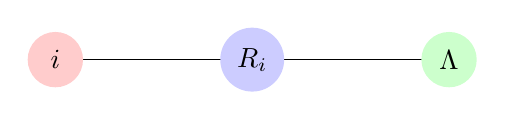
\begin{tikzpicture}[scale=0.25]
\draw (0,0) -- (20,0);
\draw (20,0) node[minimum size=2em,circle,fill=green!20] {$\Lambda$};
\draw (0,0) node[minimum size=2em,circle,fill=red!20] {$i$};
\draw (10,0) node[minimum size=2em,circle,fill=blue!20] {$R_{i}$};
\end{tikzpicture}
\end{center}
\end{figure}
\medskip
\item A socio-economic role is a reflection of the governance system ($\Lambda$) that an agent exists within: includes behavioural rules, cultural norms, media that are associated with specialisations.
\medskip
\item Economic agents adopt a socio-economic role through either \emph{adaptive specialisation} or \emph{objective specialisation}.
\end{itemize}
\end{frame}


\begin{frame} %\frametitle{}
\begin{itemize}
\item The fundamental problem of the Core needs to be resolved through the use of institutional mechanisms.
\end{itemize}
\medskip
\begin{figure}[h]
\begin{center}
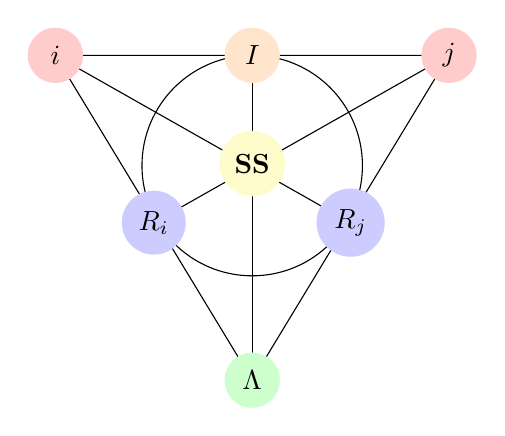
\begin{tikzpicture}[scale=0.25]
\draw (0,17) -- (10,0.5) -- (20,17) -- (0,17);
\draw (10,0.5) -- (10,17);
\draw (0,17) -- (15,8.5);
\draw (20,17) -- (5,8.5);
\draw (10,11.4) circle (5.6cm) ;
\draw (10,0.5) node[minimum size=2em,circle,fill=green!20] {$\Lambda$};
\draw (0,17) node[minimum size=2em,circle,fill=red!20] {$i$};
\draw (20,17) node[minimum size=2em,circle,fill=red!20] {$j$};
\draw (10,17) node[minimum size=2em,circle,fill=orange!20] {$I$};
\draw (5,8.5) node[minimum size=2em,circle,fill=blue!20] {$R_i$};
\draw (15,8.5) node[minimum size=2em,circle,fill=blue!20] {$R_j$};
\draw (10,11.5) node[minimum size=2em,circle,fill=yellow!20] {\textbf{SS}};
\end{tikzpicture}
\end{center}
\end{figure}
\begin{itemize}
\medskip
\item Due to the problem of the Core economic agents are considered as \emph{centrifugal} forces and the governance system as a \emph{centripetal} force.
\end{itemize}
\end{frame}


\begin{frame} %\frametitle{}
\begin{itemize}
\item The formation of economic relationships leads to a global social structure termed as an \emph{interaction infrastructure}.
\medskip
\item Specifically, an interaction infrastructure refers to a tuplee consisting of:
\begin{itemize}
\medskip
\item[1.] A population of consumer-producers; and
\medskip
\item[2.] A set of functional bilateral economic interactions and relationships formed between the population of consumer-producers.
\end{itemize}
\medskip
\item Interaction infrastructures are represented as \emph{networks}.
\medskip
\ietm Leads to the modelling Lemma regarding the positional attributes of economic agents: Economic agents have a relational position within an interaction infrastructure. These positional attributes are derived from the economic interactions they form with others.
\end{itemize}
\end{frame}

\subsection{Growth and development of the socio-economic space}

\begin{frame} \frametitle{Chapter 3: Growth and development of the socio-economic space}
\begin{itemize}
\item All economic relationships and interactions are socially embedded and exist within some well-defined space. We term this interaction space as a \textbf{socio-economic space}.
\medskip
\item A socio-economic space refers to a given set of economic agents engaged in a well-described collection of general economic interactions that operate under a well-defined collection of media and institutions.
\medskip
\item As such the socio-economic space contains economic agents, interaction infrastructures, and a governance system guiding the formation of these relationships.
\medskip
\ietm This chapter provides an overview of the socio-economic space and, with it, an analysis and simulation of its growth and development through adaptive specialisation.
\end{itemize}
\end{frame}

\begin{frame} %\frametitle{}
\begin{figure}[h]
\centering
\includegraphics[scale=0.15]{../Images/structure-space.png}
\end{figure}
\begin{itemize}
\item There exists a two-way relationship between the population of economic agents, their relational position within the economy, and the set of institutions in the governance system.
\end{itemize}
\end{frame}

\begin{frame} %\frametitle{}
\begin{itemize}
\item The socio-economic space is defined in a formal manner as a mathematical concept. Allows us to discuss these concepts in a more well-defined way.
\medskip
\item For a given collection of media and institutions, a socio-economic space can be represented by a pair $(N, \mathcal{G})$ where $N = \{1, \ldots, n\}$ is a given set of economic agents and
\begin{equation*}
\mathcal{G} \subset \mathcal{S}(N) \cup \mathcal{H}(N)
\end{equation*}
is a given collection of \textbf{general economic interactions} on $N$, where
\begin{equation*}
\mathcal{S}(N) = \{ S ~ \mid ~ S \subset N \mbox{ and } S \neq \varnothing \}
\end{equation*}
is the family of non-empty coalitions in the population $N$, representing \textbf{lateral} economic interactions on $N$, and
\begin{equation*}
\mathcal{H}(N) = \bigcup_{k = 2}^{\infty} N^{k}
\end{equation*}
is the class of all finite ordered sequences of economic agents, representing authority chains or \textbf{hierarchical} economic interactions in $N$.
\end{itemize}
\end{frame}

\begin{frame} %\frametitle{}
\begin{itemize}
\item Whilst discussing the evolution of the socio-economic space we distinguish the notions of growth and development.
\medskip
\item The \textbf{growth} of a socio-economic space refers to a change in some fundamental or pre-existing parameters that define the socio-economic space such that the aggregate utility of all economic agents increases.
\medskip
\item The \textbf{development} of a socio-economic space refers to a productive change in the elements of the governance system and its derived structure such that the new institutional mechanisms, for example, produces an increase in aggregate utility.
\medskip
\item \textbf{Decline} and \textbf{regression} are polar notions to growth and development.
\end{itemize}
\end{frame}

\begin{frame} %\frametitle{}
\begin{itemize}
\item Whilst discussing the evolution of the socio-economic space we distinguish the notions of growth and development.
\medskip
\item The \textbf{growth} of a socio-economic space refers to a change in some fundamental or pre-existing parameters that define the socio-economic space such that the aggregate utility of all economic agents increases.
\medskip
\item The \textbf{development} of a socio-economic space refers to a productive change in the elements of the governance system and its derived structure such that the new institutional mechanisms, for example, produces an increase in aggregate utility.
\medskip
\item \textbf{Decline} and \textbf{regression} are polar notions to growth and development.
\end{itemize}
\end{frame}

\end{document}
